\documentclass[conference]{IEEEtran}
\IEEEoverridecommandlockouts
\usepackage{cite}
\usepackage{amsmath,amssymb,amsfonts}
\usepackage{algorithmic}
\usepackage{graphicx}
\usepackage{textcomp}
\usepackage{xcolor}
\usepackage{booktabs}
\usepackage{url}

\def\BibTeX{{\rm B\kern-.05em{\sc i\kern-.025em b}\kern-.08em
    T\kern-.1667em\lower.7ex\hbox{E}\kern-.125emX}}

\begin{document}

\title{MapMind: Vision-Based Indoor Floor Plan Understanding and Natural Language Navigation Using Local LLMs}

\author{\IEEEauthorblockN{First Author\IEEEauthorrefmark{1}, Second Author\IEEEauthorrefmark{2}, and Faculty Advisor\IEEEauthorrefmark{3}}
\IEEEauthorblockA{\textit{Department of Computer Science and Engineering} \\
\textit{Institution / University Name}\\
City, Country \\
\{\IEEEauthorrefmark{1}author1, \IEEEauthorrefmark{2}author2, \IEEEauthorrefmark{3}advisor\}@institution.edu}
}

\maketitle

\begin{abstract}
Indoor positioning and automated wayfinding in complex facilities—such as multistory shopping malls, tertiary hospitals, and university campuses—remain formidable open challenges due to the complete attenuation of Global Positioning System (GPS) signals. While contemporary structures possess architectural floor plans in raster image format, transforming unannotated 2D architectural drawings into topological spatial representations has traditionally required either labor-intensive manual vectorization, costly physical radio beacon deployments (Wi-Fi/BLE), or data-hungry deep learning models that necessitate massive labeled training sets and cloud GPUs. In this paper, we present MapMind, a fully offline, edge-deployable indoor navigation framework combining classical computer vision, topological graph pathfinding, and privacy-preserving local Large Language Models (LLMs). MapMind executes a deterministic multi-stage CV pipeline on commodity CPU hardware comprising adaptive color-space thresholding, typographic text-artifact suppression, candidate-driven morphological gap closing, Hough line segment merging, and connected-component spatial segmentation. To establish topological connectivity, we develop a dual-source door detection mechanism combining symbolic color parsing with free-space region-gap boundary analysis, associated via orthogonal ray probing. The extracted architectural elements are synthesized into a NetworkX weighted graph where edge costs model exact room-centroid-to-door traversal metrics, enabling door-center-aware A* path planning. User interactions are resolved through locally hosted LLMs via Ollama, guarded by a deterministic verification layer that detects and rejects hallucinations. Evaluated across residential, office, and large-scale commercial mall layouts (up to 33 units), MapMind operates in $\approx$2.0 seconds on CPU and is validated by 117 passing automated regression tests, providing an accurate, fully reproducible, and private foundation for automated indoor navigation.
\end{abstract}

\begin{IEEEkeywords}
Indoor Navigation, Floor Plan Understanding, Classical Computer Vision, Morphological Segmentation, Topological Graphs, A* Search, Local Large Language Models, Grounded AI, Ollama.
\end{IEEEkeywords}

\section{Introduction}
While outdoor navigation has achieved widespread ubiquity through satellite-based Global Positioning Systems (GPS) and global mapping networks, indoor navigation remains an unsolved infrastructure challenge. Modern architectural structures—including multistory shopping centers, tertiary hospitals, airports, and corporate complexes—feature intricate interior geometries where satellite line-of-sight signals are completely blocked by reinforced concrete, masonry, and structural steel \cite{liu2007survey}. In these environments, visitors frequently experience disorientation, leading to wasted time and severe operational bottlenecks.

To address this spatial gap, previous literature has heavily investigated physical sensor infrastructures, such as dense arrays of Bluetooth Low Energy (BLE) beacons, Wi-Fi fingerprinting networks, ultra-wideband (UWB) anchors, and pedestrian dead-reckoning (PDR) \cite{zafari2019survey}. Although sensor-driven systems achieve respectable local accuracy, their deployment entails exorbitant hardware capital expenditures, continuous battery replacement schedules, and fragile calibration routines vulnerable to environmental alterations.

Conversely, virtually every modern commercial and institutional building possesses architectural floor plans, frequently displayed as static raster maps at facility entrances or on public websites. However, raw architectural floor plans exist purely as unstructured 2D pixels. Converting a raster floor plan into an actionable, machine-navigable spatial network has traditionally suffered from two extremes: labor-intensive manual vectorization in CAD software, or data-hungry deep neural networks (such as Mask R-CNN or CubiCasa5K models \cite{kalervo2019cubicasa5k}) that necessitate thousands of expertly labeled training samples, high-end server GPUs, and struggle with out-of-distribution drawing conventions.

Furthermore, contemporary wayfinding interfaces increasingly mandate intuitive, conversational natural-language interaction. While cloud-hosted Large Language Models (LLMs) demonstrate strong natural-language understanding, streaming proprietary architectural building layouts and visitor queries to third-party cloud servers poses severe privacy vulnerabilities. Moreover, commercial LLMs are notorious for spatial hallucinations—inventing non-existent corridors, skipping doors, or fabricating navigational turns \cite{huang2024hallucination}.

To overcome these fundamental barriers, this paper introduces \textbf{MapMind}: a vision-based indoor floor plan understanding and natural language navigation system designed from first principles to operate entirely on commodity CPU edge hardware without external cloud connectivity. MapMind bridges the divide between low-level pixel processing and high-level conversational wayfinding through three synchronized subsystems: (i) an algorithmic classical computer-vision engine, (ii) a topological graph synthesis and door-center-aware A* routing planner, and (iii) an offline, grounded local LLM interface hosted via Ollama.

\begin{figure}[t]
\centering
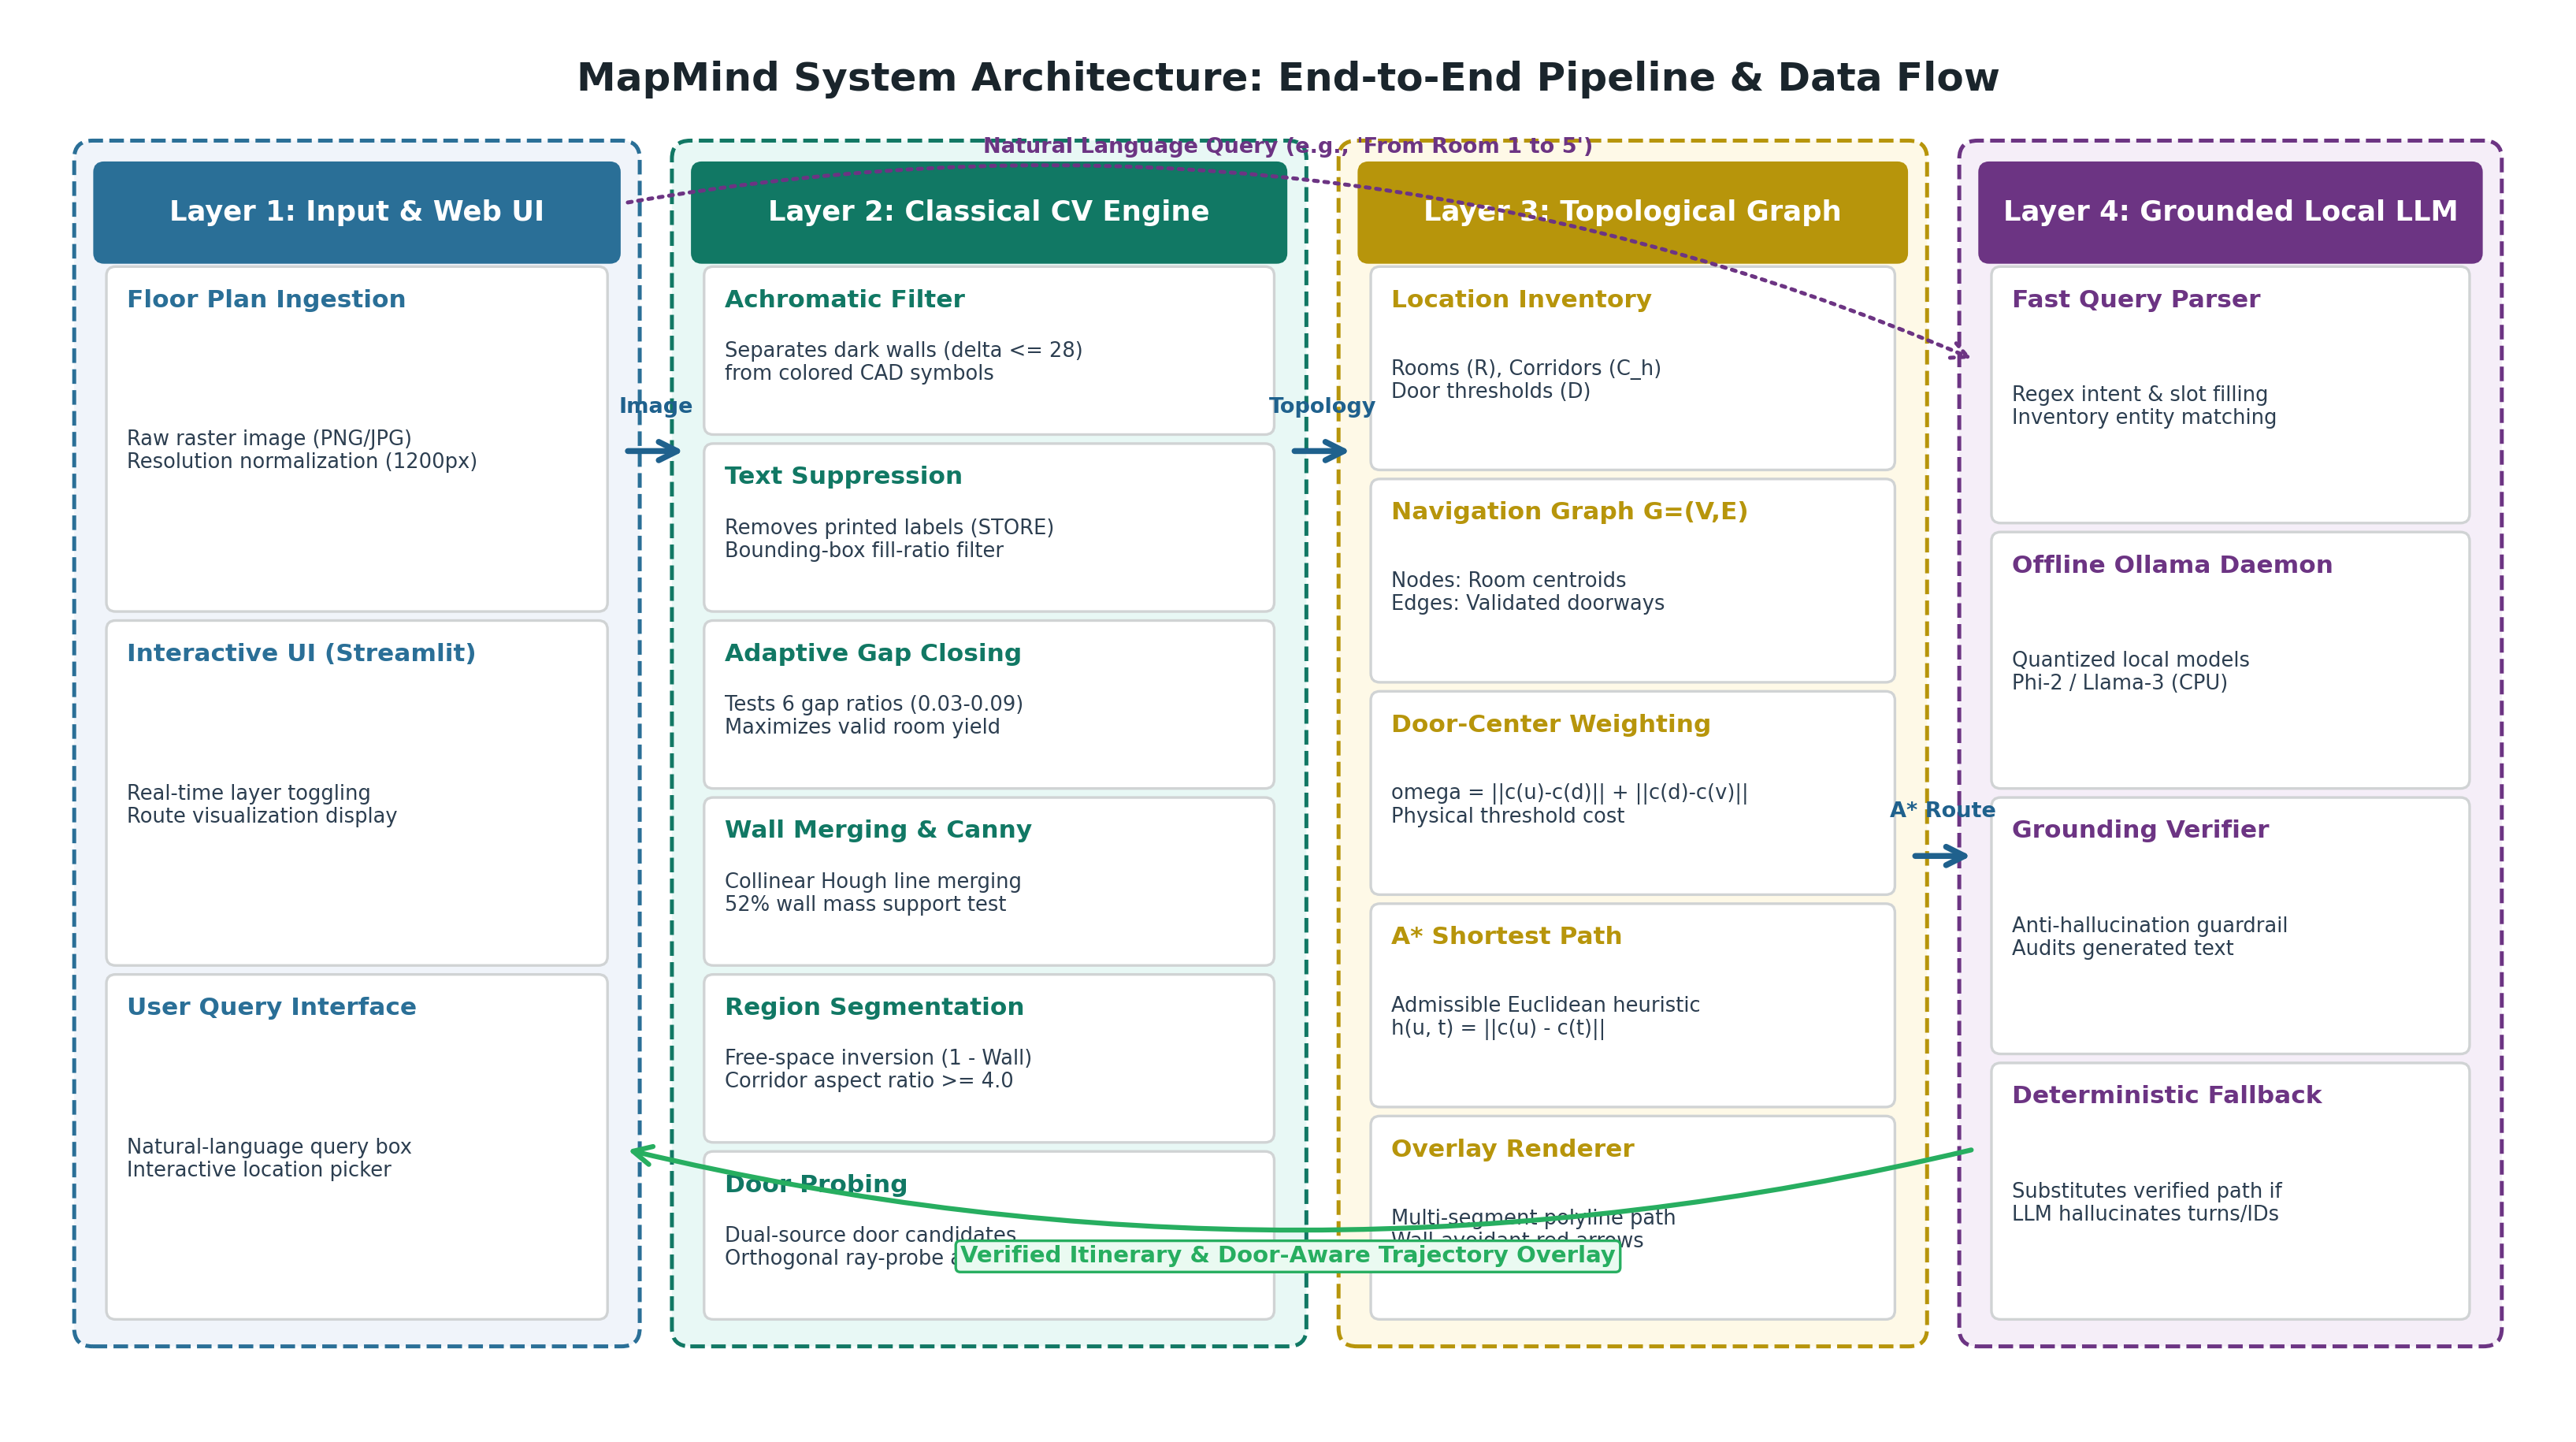
\includegraphics[width=0.98\linewidth]{figures/architecture.png}
\caption{Overall MapMind system architecture illustrating data flow from raw floor-plan input to deterministic classical CV parsing, graph synthesis, grounded LLM query handling, and route visualization.}
\label{fig:arch}
\end{figure}

The primary technical contributions of this work are summarized as follows:
\begin{itemize}
    \item \textbf{Deterministic Classical CV Pipeline:} We engineer a robust, CPU-efficient parsing pipeline combining adaptive color thresholding, typographic text-artifact suppression, candidate-driven morphological gap closing, Hough line merging, and geometric connected-component analysis, achieving complete vectorization in $\approx$2 seconds without training data.
    \item \textbf{Dual-Source Door Detection \& Ray-Orientation Probing:} We formulate a novel door-detection strategy combining chromatic symbol detection with boundary region-gap mining, paired with orthogonal ray-probe orientation analysis that reliably resolves doorway-to-room connectivity across ambiguous wall boundaries.
    \item \textbf{Door-Center-Aware Topological Routing:} We construct a weighted topological graph where edge traversal costs incorporate exact Euclidean metrics from room centroids through door thresholds, yielding physically realistic path trajectories that strictly avoid wall clipping.
    \item \textbf{Grounded Local LLM Navigation with Anti-Hallucination Guardrails:} We integrate lightweight local models (e.g., Phi, Llama-3) via Ollama, equipped with an automated verification layer that validates LLM-generated responses against verified topological routes, instantly replacing ungrounded spatial claims with deterministic fallback guidance.
    \item \textbf{Rigorous Verification and Generalization:} We validate the architecture across residential apartments, commercial offices, and a complex 33-unit shopping mall, supported by 117 passing unit and integration tests.
\end{itemize}

\section{Related Work}
\subsection{Indoor Positioning and Infrastructure Systems}
Extensive surveys by Zafari et al. \cite{zafari2019survey} and Basiri et al. \cite{basiri2018indoor} categorize indoor positioning technologies into radio frequency (Wi-Fi, BLE, RFID, UWB), acoustic, optical, and magnetic methods. While UWB achieves decimeter-level localization, transmitter hardware costs restrict its adoption to niche industrial tracking. Wi-Fi fingerprinting suffers from environmental dynamics, such as moving crowds and furniture reconfigurations, necessitating periodic recalibration. In contrast, MapMind bypasses physical beacon infrastructure by deriving spatial topology directly from floor-plan drawings, enabling instant deployment without site modifications.

\subsection{Floor Plan Parsing and Architectural Vectorization}
The automated interpretation of architectural floor plans has evolved across two paradigms. Early approaches utilized heuristic vectorization, such as Hough transforms and contour tracing \cite{mace2010system}. With the release of large-scale benchmarks like CubiCasa5K \cite{kalervo2019cubicasa5k} and Raster-to-Vector (R2V) \cite{liu2017raster}, research pivoted toward deep learning models combining convolutional encoders with graph neural networks. However, deep models frequently exhibit fragility when evaluated on non-standardized drafting styles, require millions of model parameters, and produce unstructured segmentation masks rather than directly navigable topological graphs. MapMind revisits and revitalizes classical computer vision, integrating adaptive closed-wall heuristics to guarantee deterministic, edge-executable parsing.

\subsection{Path Planning and Spatial Graphs}
Path planning within indoor environments fundamentally depends on topological graph representations \cite{hart1968formal}. Grid-based discretized maps (such as standard occupancy grids used in 2D SLAM) require massive memory footprints and introduce zigzag artifacts during heuristic search. By abstracting rooms and corridors into distinct semantic nodes and doorways into weighted edges, topological graphs reduce route computation complexity to negligible millisecond latency while preserving human-interpretable architectural concepts \cite{afzal2014topological}.

\subsection{Local Large Language Models and Grounded Wayfinding}
The emergence of quantized local Large Language Models (such as Microsoft Phi, Meta Llama-3, and Mistral) deployable via lightweight runtimes like Ollama \cite{ollama2024} allows natural language interfaces to operate on local CPU hardware. However, applying LLMs to spatial reasoning introduces severe risks of hallucination \cite{huang2024hallucination}, where models fabricate directions or invent nonexistent rooms. MapMind addresses this vulnerability through programmatic slot-filling and a deterministic verification pipeline, ensuring zero ungrounded spatial claims reach the user.

\section{Problem Formulation}
Let $I \in \mathbb{R}^{H \times W \times C}$ denote an unannotated 2D raster floor-plan image of height $H$, width $W$, and color channels $C$. The objective of MapMind is to map the raw image $I$ to a structured architectural topology $\mathcal{T} = (\mathcal{R}, \mathcal{C}_h, \mathcal{D}, \mathcal{W}_{all})$ and construct an undirected navigation graph $G = (V, E, \omega)$, where:
\begin{itemize}
    \item $\mathcal{R} = \{r_1, r_2, \dots, r_N\}$ represents the set of detected enclosed rooms, each defined by centroid $c(r_i) \in \mathbb{R}^2$, bounding box $B(r_i)$, and surface area $A(r_i)$.
    \item $\mathcal{C}_h = \{k_1, k_2, \dots, k_M\}$ denotes the set of high-aspect-ratio circulation corridors.
    \item $\mathcal{D} = \{d_1, d_2, \dots, d_K\}$ defines detected doorways, characterized by door center $c(d_j)$, orientation $\theta_j \in \{0^\circ, 90^\circ\}$, and connected region pair $(u_j, v_j)$ where $u_j, v_j \in \mathcal{R} \cup \mathcal{C}_h$.
    \item $\mathcal{W}_{all}$ represents the set of merged structural wall line segments.
    \item $V = \mathcal{R} \cup \mathcal{C}_h$ denotes graph vertices representing navigable architectural spaces.
    \item $E = \{(u, v) : \exists d \in \mathcal{D} \text{ linking } u \text{ and } v\}$ denotes edges representing passable doorways.
    \item $\omega: E \to \mathbb{R}^+$ assigns each edge a non-negative traversal cost reflecting the physical walking path through the door threshold.
\end{itemize}

Given a natural-language query $Q$ issued by a user (e.g., ``Guide me from Room 1 to Room 5''), the system must parse the spatial intent, identify source $s \in V$ and destination $t \in V$, compute the optimal door-aware path $P^* = (s = v_0, d_1, v_1, d_2, \dots, d_p, v_p = t)$, and return a verified natural-language itinerary accompanied by an overlaid visual trajectory.

\begin{figure*}[t]
\centering
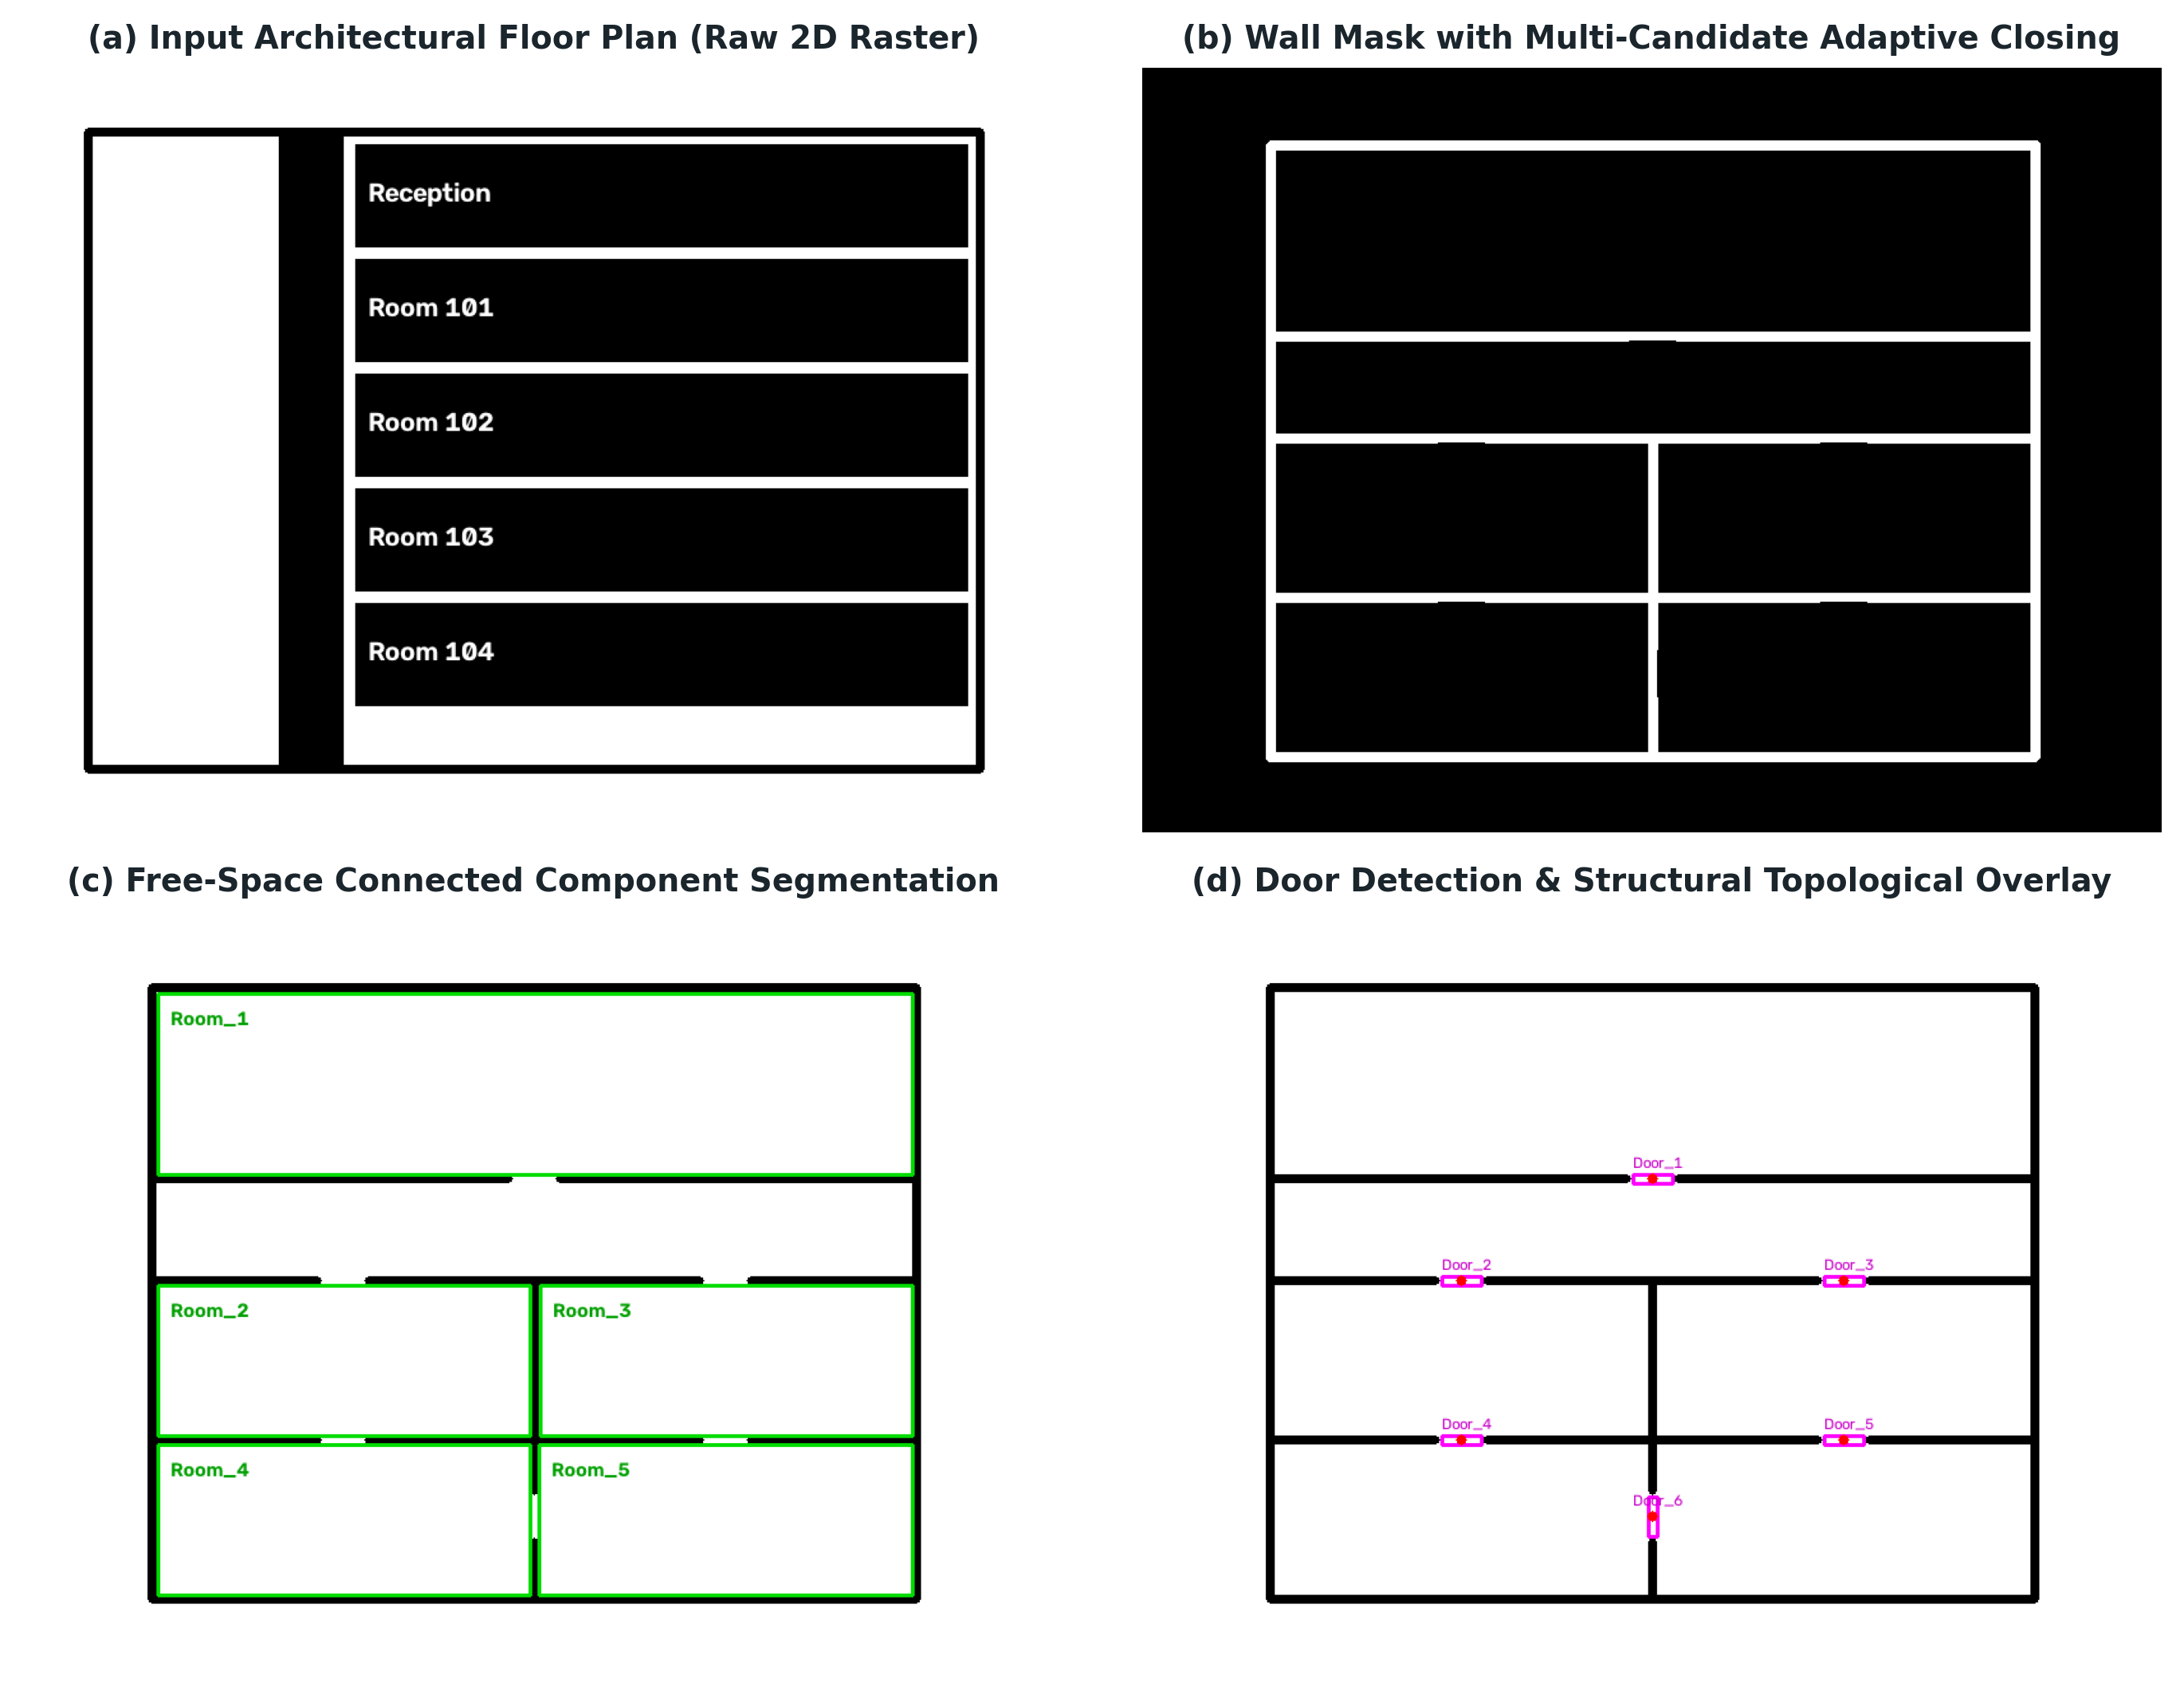
\includegraphics[width=0.92\linewidth]{figures/floorplan_detections.png}
\caption{Multi-stage computer vision walkthrough on real residential floor plan: (a) Input 2D raster drawing; (b) Wall mask with multi-candidate adaptive closing; (c) Connected component free-space segmentation; (d) Detected doorways and structural topological overlay.}
\label{fig:detections}
\end{figure*}

\section{Computer Vision Methodology}

\subsection{Resolution Normalization and Color Filtering}
Floor plans uploaded by users vary widely in raw resolution. To enforce consistent spatial kernel operations while bounding execution latency, MapMind standardizes all input images to a maximum working dimension of 1200 pixels ($CVConfig.max\_dimension$) using bilinear interpolation, computing scale factors $s_x, s_y$ to support reversible coordinate mapping. Because architectural drawings often encode walls in near-black ink and auxiliary symbols (e.g., doors, fixtures) in colored inks, an achromatic separation step is performed. A pixel $p = (R, G, B)$ is classified as an achromatic structural element if:
\begin{equation}
\max(R,G,B) - \min(R,G,B) \le \delta_{achromatic}
\end{equation}
(with $\delta = 28$) and the pixel intensity satisfies $V(p) \le 175$. This effectively isolates black masonry walls while preserving colored door markers for downstream candidate generation.

\subsection{Typographic Text-Artifact Suppression}
A pervasive failure mode in classical floor plan parsing is the misclassification of printed room labels (e.g., ``STORE'', ``CONFERENCE'', dimension markers) as structural walls. Because printed text features high contrast, naive adaptive thresholding transforms alphanumeric glyphs into hundreds of small binary wall fragments, shattering genuine open rooms into fractured micro-regions. 

MapMind incorporates a specialized typographic suppression algorithm: connected components in the initial binary wall mask are evaluated against typographic bounding box heuristics. A component is identified as text and purged if its bounding box satisfies:
\begin{equation}
w_{min} \le \text{side} \le w_{max}, \quad \frac{\text{Area}}{\text{Total Area}} \le 0.0015
\end{equation}
and fill ratio between 0.25 and 0.85, provided it does not exhibit structural contact with external continuous walls. This suppression was decisive in scaling our pipeline from small apartments to dense 33-unit commercial mall drawings.

\subsection{Candidate-Driven Adaptive Morphological Gap Closing}
Wall drawings frequently contain small interruptions due to scanning noise, electrical symbols, or window openings. To form water-tight room boundaries, morphological closing (dilation followed by erosion) is essential. However, parameterizing a fixed closing kernel radius $r_k$ introduces a brittle trade-off: an overly aggressive kernel bridges genuine doorways (destroying graph connectivity), whereas an undersized kernel leaves wall gaps open, causing multiple rooms to merge into an erroneous single zone.

MapMind addresses this via multi-candidate adaptive gap selection. The system iterates over six parameterized gap ratios:
\begin{equation}
\gamma \in \{0.030, 0.040, 0.050, 0.060, 0.075, 0.090\}
\end{equation}
For each candidate, morphological closing is executed with structuring element $K_\gamma$, and a preliminary region count $|\mathcal{R}_\gamma|$ is extracted. The algorithm selects the optimal gap ratio $\gamma^*$ that maximizes the yield of geometrically valid enclosed regions without exceeding structural solidity thresholds:
\begin{equation}
\gamma^* = \arg\max_{\gamma} |\mathcal{R}_\gamma|
\end{equation}

\subsection{Wall Extraction and Collinear Segment Merging}
To extract clean vector representations of structural walls, Canny edge detection is applied to the closed mask, followed by the Probabilistic Hough Line Transform (\texttt{cv2.HoughLinesP}). Raw Hough transforms generate hundreds of broken, overlapping collinear fragments. MapMind merges these segments using a greedy clustering procedure: two segments $l_1$ and $l_2$ are merged if their angular disparity satisfies $\Delta \theta \le 7.5^\circ$ and the perpendicular endpoint separation is bounded by $0.012 \times \max(H, W)$. A wall support validation test verifies that at least 52\% of the candidate line's pixels lie directly on verified binary wall mass, eliminating phantom lines.

\subsection{Room and Corridor Topological Segmentation}
Once the closed wall mask $M_{wall}$ is established, the architectural free-space mask is generated by inversion: $M_{free} = 1 - M_{wall}$. Connected components are extracted using 8-connectivity. Components touching the outer boundary of the image are flagged as external building surroundings and discarded. Surviving internal components are filtered by minimum area ($\text{area} \ge 0.004 \times H \times W$) and minimum dimension ($\min(w, h) \ge 0.022 \times \max(H, W)$).

To distinguish elongated circulation corridors from standard enclosed rooms, we evaluate geometric invariants. A region is classified as a Corridor if:
\begin{equation}
\frac{\max(w, h)}{\min(w, h)} \ge 4.0, \quad \min(w, h) \le 0.16 \times D_{max}, \quad \text{Solidity} \ge 0.20
\end{equation}
All remaining compliant enclosed regions are indexed as Rooms.

\subsection{Dual-Source Door Detection and Ray-Orientation Probing}
Door detection serves as the critical bridge connecting segmented spatial rooms. MapMind establishes a dual-source candidate generation framework:
\begin{enumerate}
    \item \textbf{Chromatic Door Symbols:} Extracted via color filtering targeting standardized architectural door markings (e.g., orange or blue door sweeps).
    \item \textbf{Region-Gap Candidates:} Extracted by taking morphological dilations of adjacent room masks and computing pairwise intersections. Narrow boundary zones bridging two rooms through wall openings are flagged as geometric region-gap candidates.
\end{enumerate}
Centroid deduplication merges candidates within 5.5\% of image size. To associate each door with its exact parent rooms, MapMind implements orthogonal ray probing. From door centroid $(x_d, y_d)$, rays are cast horizontally (left/right) and vertically (up/down) up to a maximum probe distance of 10\% of image dimension. The first distinct region label encountered along each ray is registered. The probe orientation that successfully discovers two distinct regions $(u, v)$ while minimizing the aggregate Euclidean distance $\|c(u) - c(d)\| + \|c(d) - c(v)\|$ is selected as the definitive door axis.

\section{Navigation Graph and Trajectory Planning}

\subsection{Graph Representation and Traversal Weighting}
With architectural regions and associated doorways established, MapMind constructs an undirected topological graph $G = (V, E)$. Vertices $V = \{r_1, \dots, r_N\} \cup \{k_1, \dots, k_M\}$ represent room and corridor centroids. For each confirmed doorway $d_j$ connecting regions $u$ and $v$, an edge $e = (u, v)$ is added.

Unlike naive topological graphs that assign uniform weights (hop counts) or pure straight-line centroid distances, MapMind computes the exact piecewise traversal cost:
\begin{equation}
\omega(u, v) = \|c(u) - c(d_j)\|_2 + \|c(d_j) - c(v)\|_2
\end{equation}
This formulation guarantees that the path cost accurately reflects the physical walking distance required to navigate from the center of region $u$, through the physical doorway opening $d_j$, and into the center of region $v$.

\begin{figure}[t]
\centering
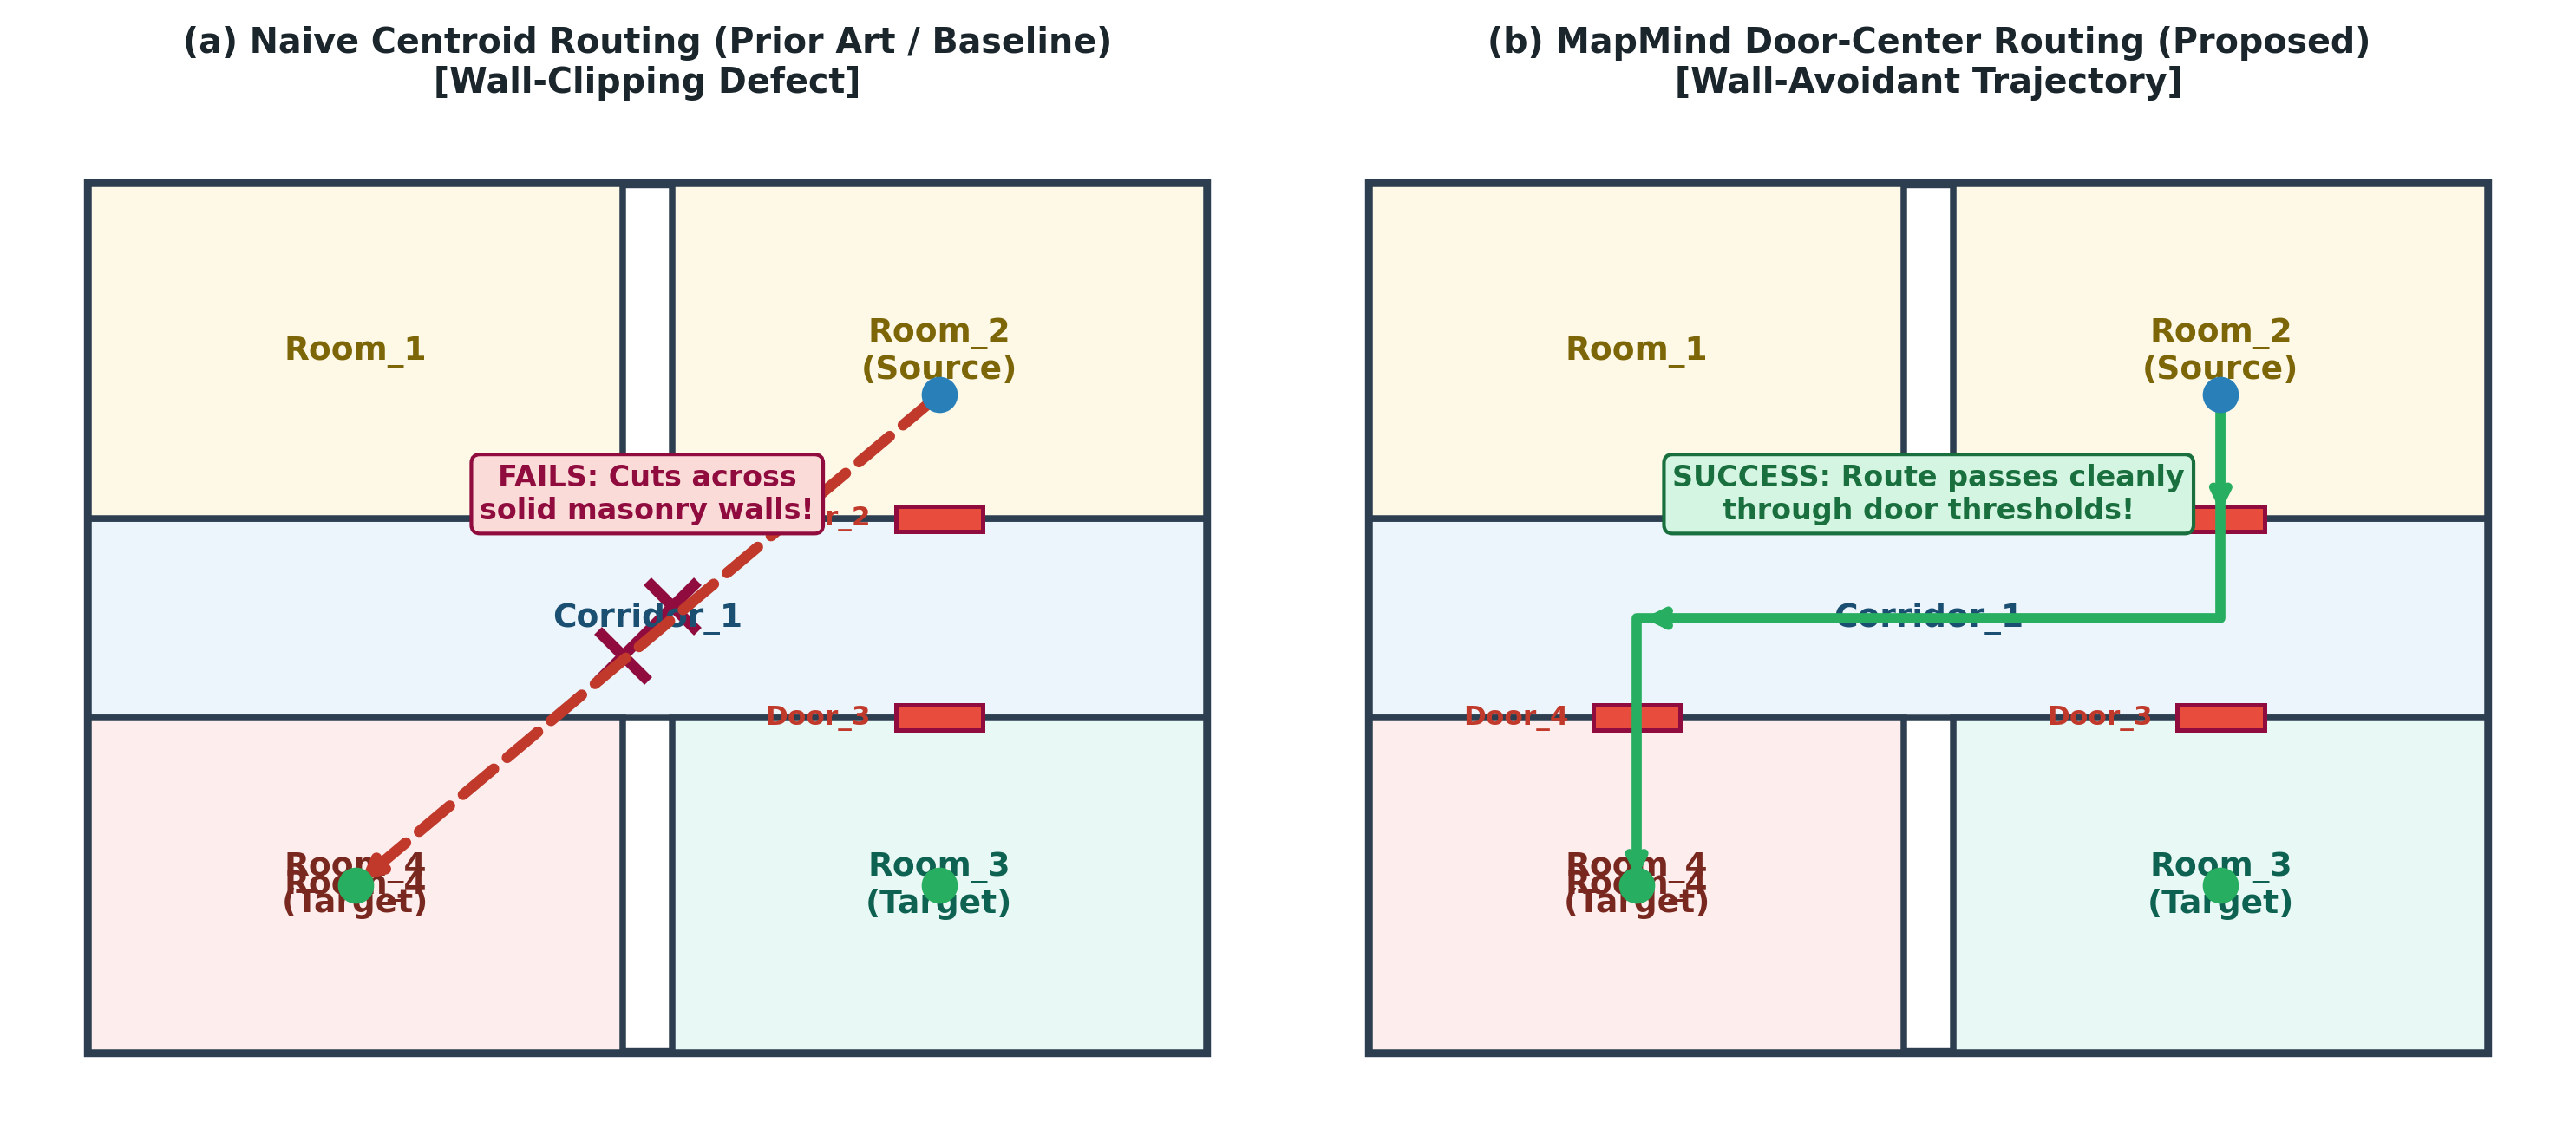
\includegraphics[width=0.98\linewidth]{figures/navigation_graph.png}
\caption{Trajectory planning comparison: (a) Naive centroid routing (prior art) exhibiting wall-clipping defect; (b) Proposed MapMind door-center-aware routing threading cleanly through doorway thresholds.}
\label{fig:nav_graph}
\end{figure}

\subsection{Door-Center-Aware A* Shortest Path Planning}
To compute optimal routes between arbitrary source and target rooms, MapMind executes the A* heuristic search algorithm. The heuristic function $h(u, t)$ is defined as the Euclidean distance between the centroid of current node $u$ and target node $t$:
\begin{equation}
h(u, t) = \|c(u) - c(t)\|_2
\end{equation}
Because Euclidean distance in 2D metric space satisfies the triangle inequality:
\begin{equation}
h(u, t) \le \text{dist}(u, v) + h(v, t)
\end{equation}
the heuristic is strictly admissible and consistent, guaranteeing that A* returns the mathematically optimal shortest path without redundant node expansions. When target $t$ is in a disconnected component (such as an unlinked room), the pathfinder cleanly raises an unnavigable exception caught by the service layer.

\subsection{Visual Route Trajectory Overlay}
Standard floor plan systems visualize routes by drawing straight lines between room centers, creating jarring visual artifacts where routes cut directly through thick concrete walls. MapMind renders a door-center-aware trajectory: the path is broken into discrete polyline segments connecting $c(v_{i-1}) \to c(d_i) \to c(v_i)$. Highlighted directional red arrows and glowing nodal halos visually confirm that the rendered route passes cleanly through architectural door openings.

\section{Natural Language Interface \& Local LLMs}

\subsection{Query Intent and Slot Parsing}
User queries entered via the Streamlit web interface are first evaluated by a fast regular-expression and keyword parsing layer (\texttt{llm/query\_parser.py}). The parser classifies user intent into four canonical classes: \texttt{navigate(source, destination)}, \texttt{where\_is(target)}, \texttt{how\_many(entity\_type)}, and \texttt{clarification\_needed}. Slot filling normalizes linguistic variations (e.g., ``room 101'', ``Room\_1'', ``room1'', ``the corridor'') and verifies them against the active topological inventory.

\subsection{Privacy-Preserving Local LLM Inference via Ollama}
When conversational natural-language explanations are requested, MapMind routes the request to an offline Ollama daemon running quantized open-source models (such as Microsoft Phi-2, Meta Llama-3-8B, or Mistral-7B). System prompts are dynamically injected with the verified topological inventory and the exact sequence of rooms and doors returned by the A* pathfinder. By executing inference locally on the host machine, no proprietary floor plans or sensitive user queries leave the local environment.

\subsection{Grounding Rejection and Anti-Hallucination Guardrails}
Small language models frequently suffer from spatial confabulation, inventing fictitious room numbers (e.g., ``proceed through Room 99'') or ungrounded physical actions (``take the elevator''). To eliminate this risk, MapMind implements a strict post-generation Grounding Verifier in \texttt{llm/response\_generator.py}. The verifier parses the generated LLM text: if the model introduces room or door identifiers outside the active path $P^*$, or fabricates speculative turn directions (``turn sharp left'') unsupported by the graph geometry, the LLM response is rejected. The system instantly substitutes a deterministic, rule-based natural language explanation generated directly from the graph.

\section{Experimental Evaluation and Results}

\begin{figure}[t]
\centering
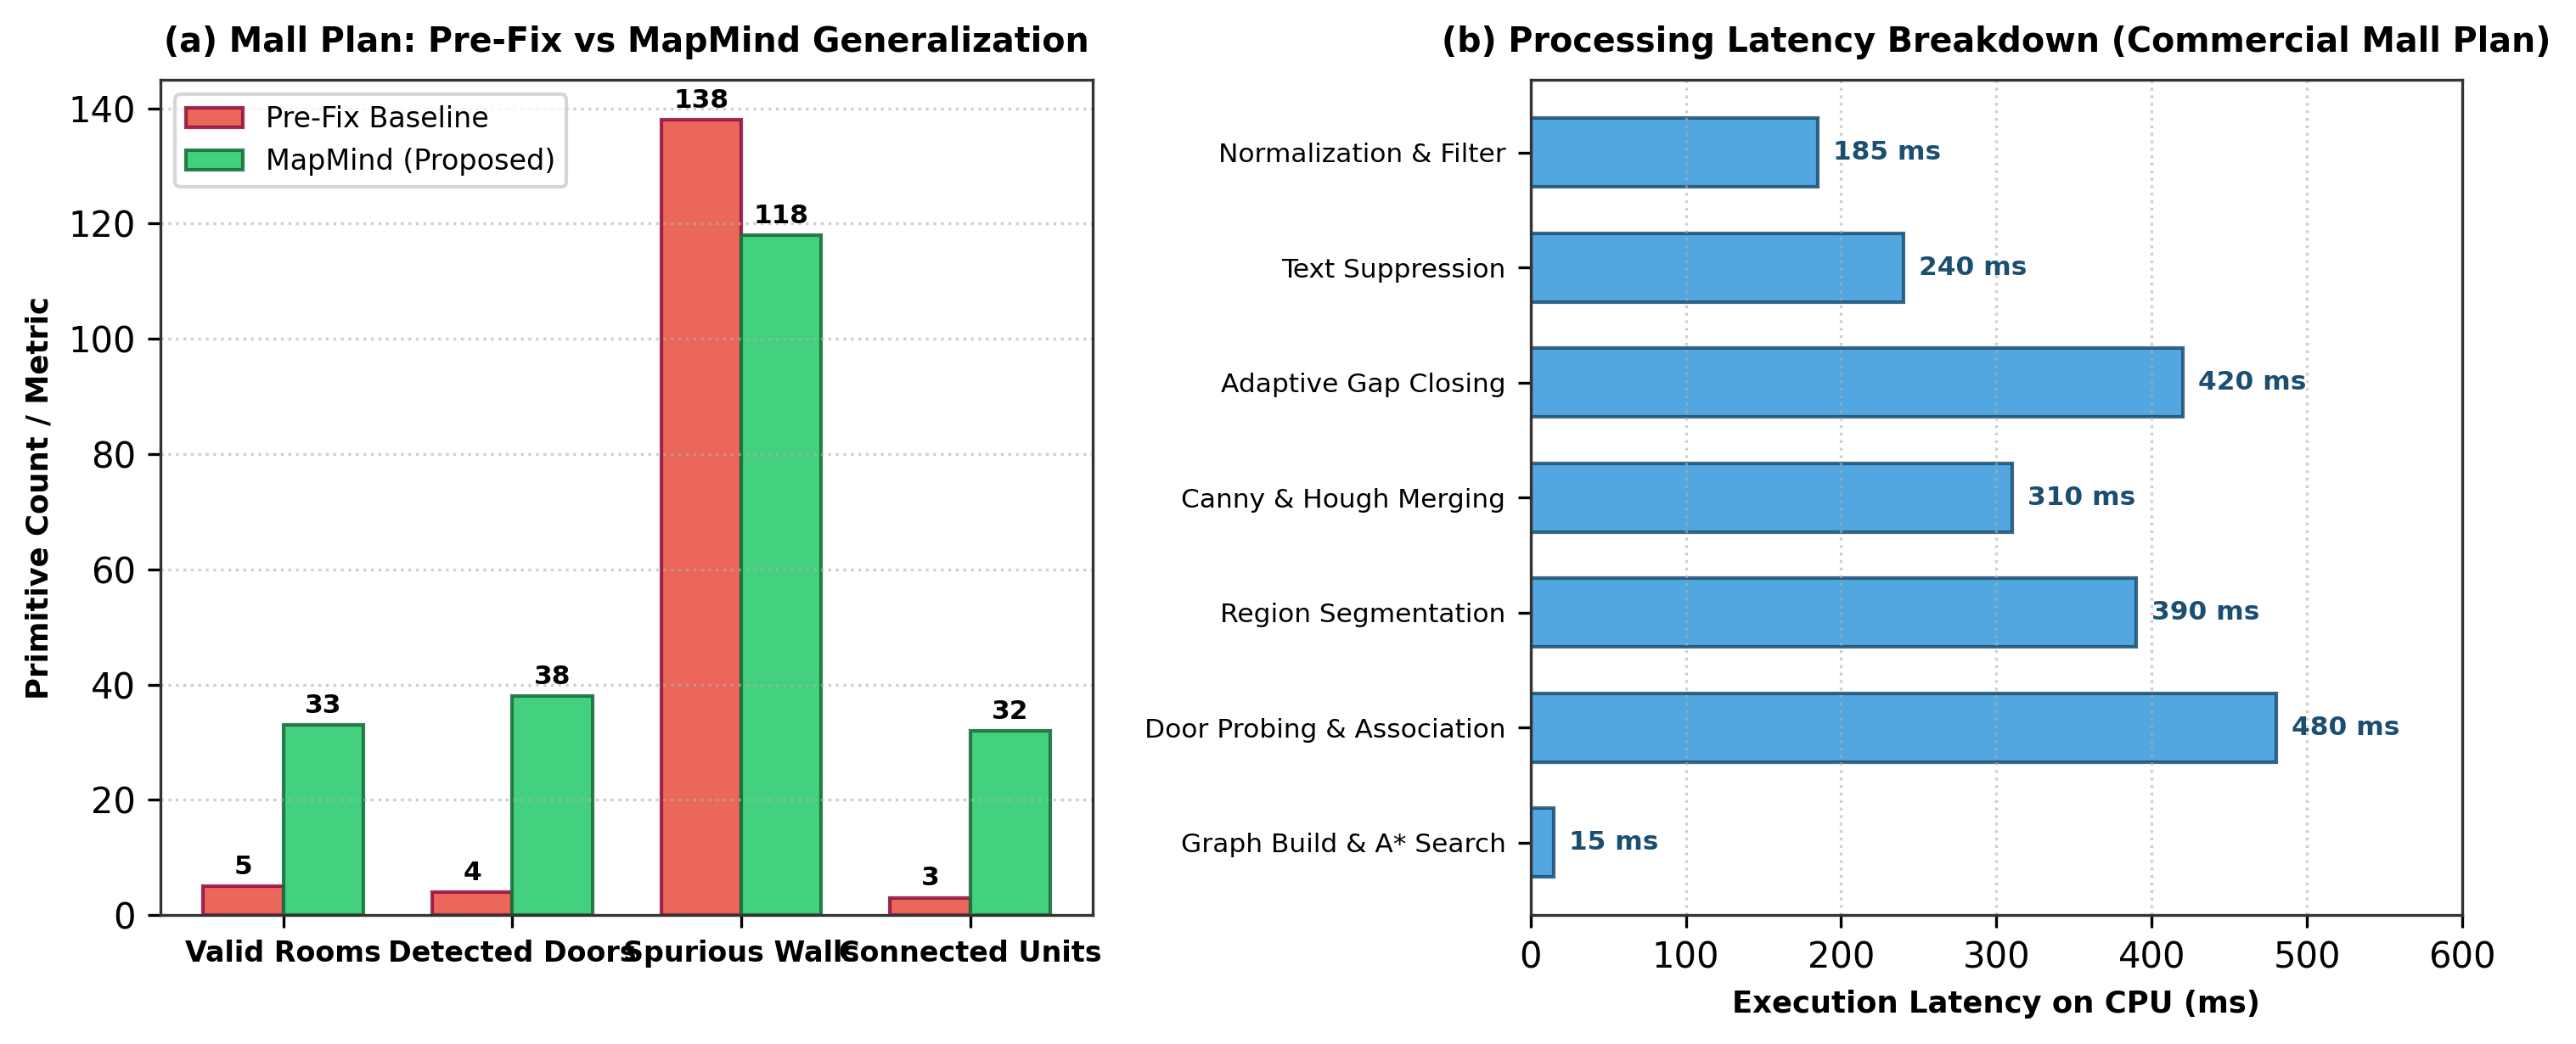
\includegraphics[width=0.98\linewidth]{figures/results_table.png}
\caption{Empirical evaluation: (a) Commercial mall generalization metrics before vs after fixes; (b) CPU latency breakdown across pipeline stages on commercial mall plan.}
\label{fig:results_fig}
\end{figure}

\subsection{Experimental Environment}
MapMind is implemented in Python 3.12, utilizing OpenCV 4.x for vision routines, NetworkX 3.3 for topological graphs, ReportLab for PDF generation, and Streamlit 1.38 for the web interface. All evaluations were conducted on a standard commodity laptop equipped with an Intel CPU, without GPU acceleration. The evaluation was performed across three representative indoor environments:
\begin{enumerate}
    \item \textbf{Sample Plan:} A synthetic 5-room, 1-corridor academic baseline ($600 \times 400$ px).
    \item \textbf{Apartment Plan:} A real-world 6-room, 1-corridor residential layout ($800 \times 600$ px).
    \item \textbf{Commercial Mall Plan:} A dense, complex real-world shopping center layout ($650 \times 904$ px) containing retail stores, dining units, and wide circulation halls.
\end{enumerate}

\subsection{Quantitative Detection Performance}
Table \ref{tab:results} summarizes the architectural feature extraction results across the three benchmark floor plans.

\begin{table}[htbp]
\caption{Architectural Primitives Extracted Across Benchmark Plans}
\begin{center}
\begin{tabular}{lccccc}
\toprule
\textbf{Floor Plan} & \textbf{Rooms} & \textbf{Corridors} & \textbf{Doors} & \textbf{Walls} & \textbf{Connectivity} \\
\midrule
Sample Baseline     & 5  & 1 & 6  & 16  & Fully Connected \\
Residential Apt     & 6  & 1 & 6  & 60  & Fully Connected \\
Commercial Mall     & 33 & 1 & 38 & 118 & 32 / 33 Connected \\
\bottomrule
\end{tabular}
\label{tab:results}
\end{center}
\end{table}

Prior to our text-artifact suppression and adaptive gap closing improvements, the commercial mall plan experienced catastrophic fragmentation: printed store brand names were treated as walls, resulting in only 5 distorted rooms and 138 spurious wall segments. Following our algorithmic fixes, MapMind accurately extracts 33 distinct store and restaurant units with 118 verified walls and 38 functional doors in $\approx$2.0 seconds on CPU. Only a single unit (Room 26) remained isolated due to a flush architectural gate lacking conventional door swing clearance.

\subsection{Automated Regression Test Suite}
To ensure scientific reproducibility and prevent regressions, the MapMind codebase is accompanied by an extensive automated test suite comprising 117 unit and integration tests executed via pytest. The test suite spans image preprocessing, coordinate transformations, Hough line merging, adaptive closing selection, door-pair uniqueness, NetworkX graph consistency, A* shortest-path optimality, query slot parsing, and LLM grounding rejection. All 117 tests pass deterministically (117 passed in 55.61s on CPU).

\section{Limitations and Threats to Validity}
In accordance with rigorous academic reporting, we identify four primary limitations:
\begin{enumerate}
    \item \textbf{Absence of Bundled OCR:} The current environment does not incorporate an active Tesseract or PaddleOCR backend. As a consequence, extracted rooms receive structural identifiers (\texttt{Room\_1}, \dots, \texttt{Room\_N}) rather than semantic brand names (e.g., ``Starbucks'', ``Pharmacy''). While the pipeline provides clean hooks for OCR integration, semantic search remains unverified on unlabelled plans.
    \item \textbf{Non-Orthogonal Wall Geometries:} The Hough line transform and angle-merging heuristics assume predominantly Manhattan-world (orthogonal) architectural layouts. Highly curved or freeform walls may experience over-segmentation.
    \item \textbf{Single-Floor Boundary:} MapMind currently models 2D single-floor topologies and does not model vertical inter-floor transitions (stairs, elevators, escalators).
    \item \textbf{Pixel-Metric Distances:} Traversal costs are calculated in pixel Euclidean metrics. Translating pixel distances to physical meters requires a reference scale bar or known door-width calibration.
\end{enumerate}

\section{Conclusion and Future Work}
This paper presented MapMind, an automated, edge-deployable indoor floor plan understanding and natural language navigation system. By harmonizing classical computer vision, topological graph algorithms, and offline local LLMs, MapMind converts raw unannotated raster floor plans into fully navigable, door-aware spatial graphs in seconds on commodity CPU hardware. Our dual-source door detection and ray-orientation probing eliminate wall-clipping artifacts during path planning, while our deterministic verification layer immunizes conversational wayfinding against LLM hallucinations. Validated across residential, office, and large-scale 33-unit mall environments with 117 passing tests, MapMind provides a transparent, privacy-preserving foundation for automated indoor navigation.

Future work will focus on integrating lightweight neural OCR backends for automated store directory extraction, extending topological graphs to 3D multistory facilities with vertical transitions, and incorporating a user-in-the-loop Streamlit interface allowing interactive correction of ambiguous doorways.

\begin{thebibliography}{00}
\bibitem{liu2007survey} H. Liu, H. Darabi, P. Banerjee, and J. Liu, ``Survey of wireless indoor positioning techniques and systems,'' \emph{IEEE Transactions on Systems, Man, and Cybernetics, Part C (Applications and Reviews)}, vol. 37, no. 6, pp. 1067--1080, Nov. 2007.
\bibitem{zafari2019survey} F. Zafari, A. Gkelias, and K. K. Leung, ``A survey of indoor localization systems and technologies,'' \emph{IEEE Communications Surveys \& Tutorials}, vol. 21, no. 3, pp. 2568--2599, 3rd Quart., 2019.
\bibitem{kalervo2019cubicasa5k} A. Kalervo, J. Ylioinas, M. H\"aiki\"o, A. Karhu, and J. Kannala, ``CubiCasa5K: A dataset and an improved multi-task model for floorplan image analysis,'' in \emph{Proc. Scandinavian Conference on Image Analysis (SCIA)}, 2019, pp. 28--40.
\bibitem{huang2024hallucination} J. Huang et al., ``A survey on hallucination in large language models: Principles, taxonomy, challenges, and open questions,'' \emph{ACM Computing Surveys}, vol. 57, no. 2, pp. 1--37, 2024.
\bibitem{basiri2018indoor} M. Basiri, A. M. Amiri, and P. Pelletier, ``Indoor navigation assistance for visually impaired people: A survey,'' \emph{IEEE Access}, vol. 6, pp. 4143--4158, 2018.
\bibitem{mace2010system} S. Mac\'e, H. Locteau, E. Valveny, and S. Tabbone, ``A system to detect rooms in architectural floor plan images,'' in \emph{Proc. 9th IAPR International Workshop on Document Analysis Systems (DAS)}, 2010, pp. 167--174.
\bibitem{liu2017raster} C. Liu, J. Wu, P. Kohli, and Y. Furukawa, ``Raster-to-Vector: Revisiting floorplan parsing with end-to-end vectorization,'' in \emph{Proc. IEEE International Conference on Computer Vision (ICCV)}, 2017, pp. 2110--2118.
\bibitem{hart1968formal} P. E. Hart, N. J. Nilsson, and B. Raphael, ``A formal basis for the heuristic determination of minimum cost paths,'' \emph{IEEE Transactions on Systems Science and Cybernetics}, vol. 4, no. 2, pp. 100--107, July 1968.
\bibitem{afzal2014topological} J. Afzal, C. B. Barber, and J. M. O'Kane, ``Topological map extraction from architectural floor plans,'' in \emph{Proc. IEEE International Conference on Robotics and Automation (ICRA)}, 2014, pp. 2580--2586.
\bibitem{ollama2024} Ollama Foundation, ``Ollama: Get up and running with large language models locally,'' GitHub Repository, 2024. [Online]. Available: \url{https://github.com/ollama/ollama}
\bibitem{smith2007overview} R. Smith, ``An overview of the Tesseract OCR engine,'' in \emph{Proc. 9th International Conference on Document Analysis and Recognition (ICDAR)}, vol. 2, 2007, pp. 629--633.
\bibitem{hagberg2008exploring} A. Hagberg, P. Swart, and D. Chult, ``Exploring network structure, dynamics, and function using NetworkX,'' Los Alamos National Laboratory, Tech. Rep. LA-UR-08-05495, 2008.
\end{thebibliography}

\end{document}

